% uklad dokumentu
	\documentclass{article}
	\usepackage{xparse}
	\usepackage[margin=1cm]{geometry}
    \usepackage{enumerate} 
	\frenchspacing
    \linespread{1.2}
    \setlength{\parindent}{0pt}

% jezyk polski
	\usepackage[polish]{babel}
	\usepackage[utf8]{inputenc}
	\usepackage{polski}
 
% pakiety matematyczne
    \let\lll\undefined
	\usepackage{amssymb}
    \usepackage{amsthm}
	\usepackage{amsmath}
	\usepackage{amsfonts}
	\usepackage{tikz}

% hiperlacza
	\usepackage{hyperref}
	\hypersetup{
		colorlinks,
		citecolor=black,
		filecolor=black,
		linkcolor=black,
		urlcolor=black
	}

% wstawianie zdjec
	\usepackage{graphicx} 
	\pagenumbering{gobble}
	

% podstawowe informacje
    \title{Algorytmy metaheurystyczne 2}
    \author{Paweł Cegieła, Wojciech Sęk}

\begin{document} 

\maketitle

\section{Teoretyczna złożoność}
Warunkiem wyjścia w naszym algorytmie było przekroczenie $15n$ iteracji, gdzie $n=|V|$ lub $n$ ruchów bez zmiany na lepsze rozwiązanie. Rozważmy najgorszy możliwy przypadek, gdzie wykonujemy $15n$ iteracji. Niech $k$ to długość listy tabu. Implementacja listy tabu za pomocą VecDeq pozwala na dostęp do $i$-tego elementu w czasie stałym, a usuwanie i dodawanie elementów w czasie liniowym.
\\
W każdym kroku algorytmu przeglądamy wszystkich $\frac{n(n-1)}{2}$ sąsiadów danego rozwiązania i dla każdego sprawdzamy z $O(k)$ czy jest na liście tabu. Sprawdzenie o ile sąsiad zmienia wartość permutacji jest stały (dla $invert$ liczymy wcześniej z $O(n^2)$ pomocnicze tablice. Niech $O(l)$ to złożoność przybliżenia początkowego (dla 
2-$opt$ $O(n^3)$. Wybieramy najlepszego z nich. Ostatecznie mamy (dla $k$ stałego i  $2$-opta):
$$O\left(15n\cdot \frac{n(n-1)}{2} \cdot k + l\right)=O(n^3)$$


\section{Porównanie Tabu Search z 2-OPT}

\subsection{Dane z TSPLIB}

\subsubsection{Grafy asymetryczne}
\begin{center}
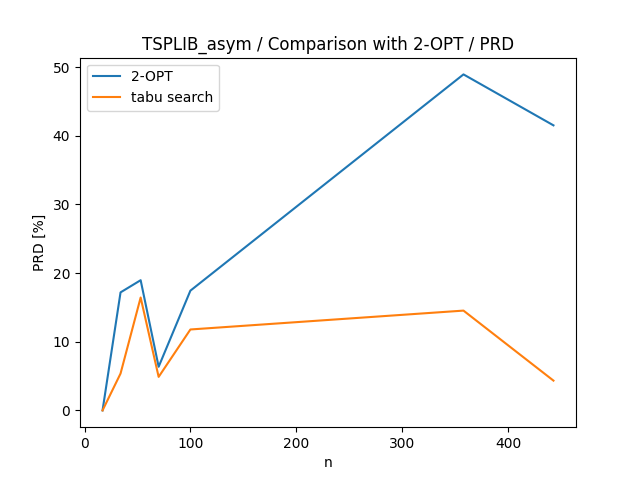
\includegraphics[width=\textwidth, 
                   height = 0.4\textheight, 
                   keepaspectratio]
                  {plots/two_opt_tsplib_asym_prd} 
\end{center}


\subsubsection{Grafy euklidesowe}

\begin{center}
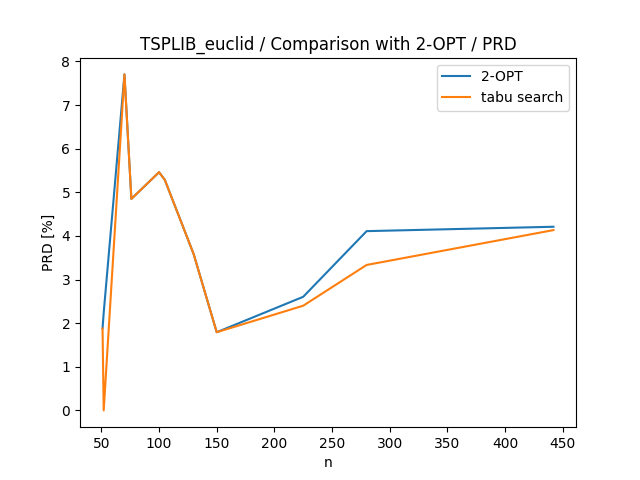
\includegraphics[width=\textwidth, 
                   height = 0.4\textheight, 
                   keepaspectratio]
                  {plots/two_opt_tsplib_euclid_prd} 
\end{center}


\subsection{Dane generowane przez nas}


\subsubsection{Grafy symetryczne}

\begin{center}
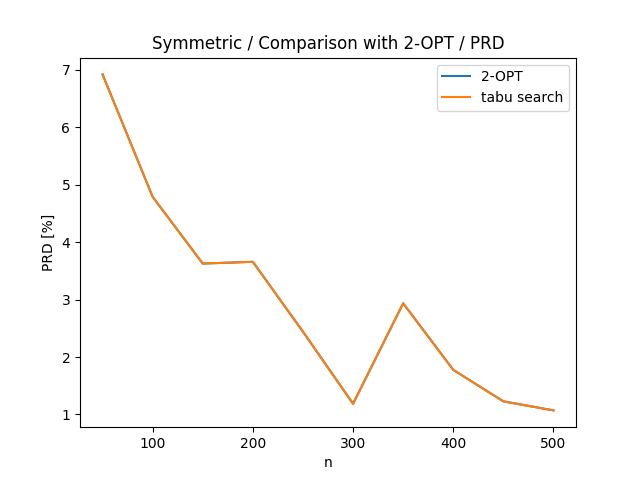
\includegraphics[width=\textwidth, 
                   height = 0.4\textheight, 
                   keepaspectratio]
                  {plots/two_opt_symmetric_prd} 
\end{center}

\subsubsection{Grafy asymetryczne}

\begin{center}
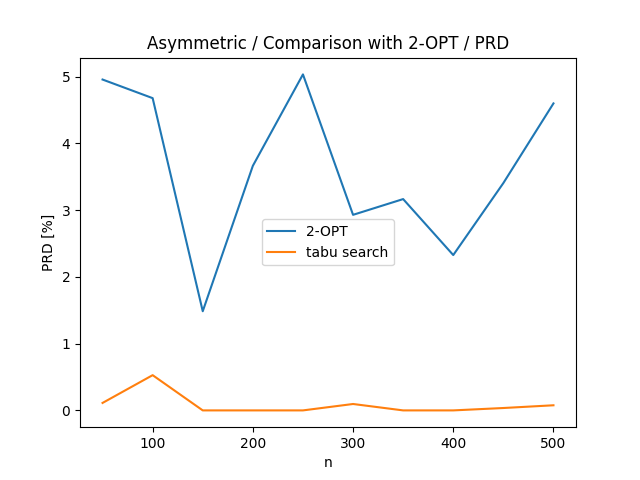
\includegraphics[width=\textwidth, 
                   height = 0.4\textheight, 
                   keepaspectratio]
                  {plots/two_opt_asymmetric_prd} 
\end{center}


\subsubsection{Grafy euklidesowe}

\begin{center}
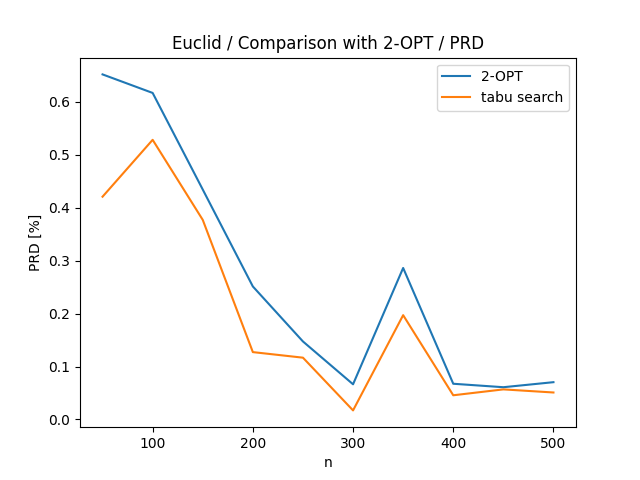
\includegraphics[width=\textwidth, 
                   height = 0.4\textheight, 
                   keepaspectratio]
                  {plots/two_opt_euclid_prd} 
\end{center}


\subsection{Obserwacje}

\subsection{Tabele}



\section{Porównanie różnych długości listy tabu}

\subsection{Dane z TSPLIB}

\subsubsection{Grafy asymetryczne}

\begin{center}
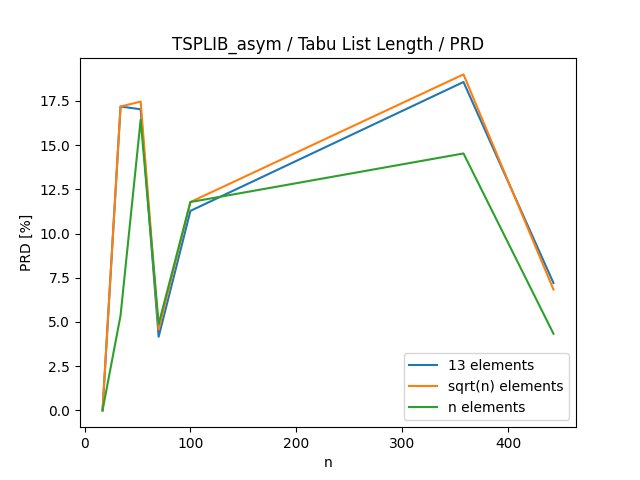
\includegraphics[width=\textwidth, 
                   height = 0.4\textheight, 
                   keepaspectratio]
                  {plots/tabu_tsplib_asym_prd} 
\end{center}

\begin{center}
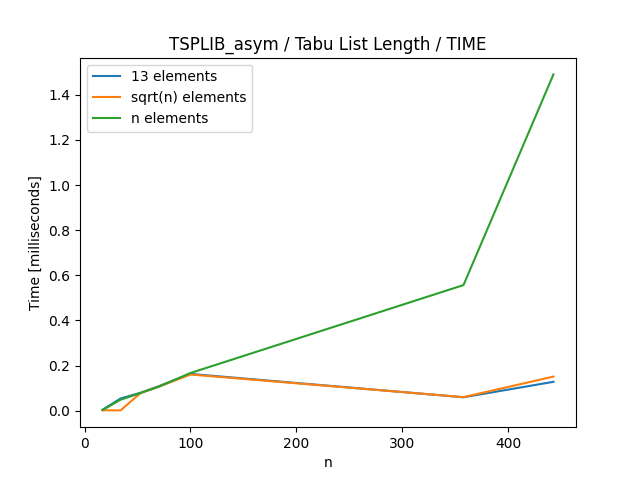
\includegraphics[width=\textwidth, 
                   height = 0.4\textheight, 
                   keepaspectratio]
                  {plots/tabu_tsplib_asym_time} 
\end{center}

\subsubsection{Grafy euklidesowe}

\begin{center}
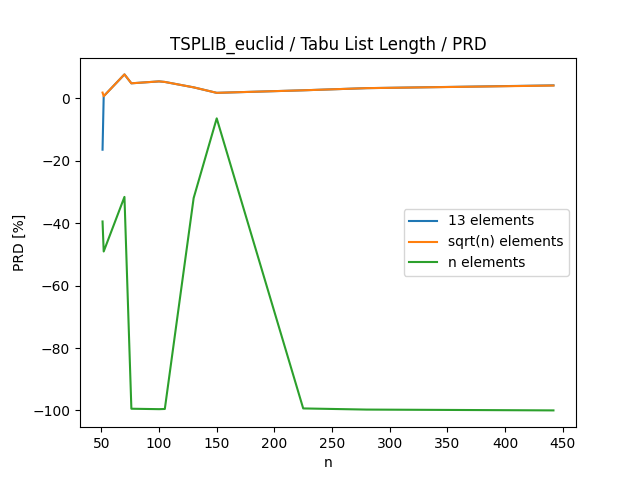
\includegraphics[width=\textwidth, 
                   height = 0.4\textheight, 
                   keepaspectratio]
                  {plots/tabu_tsplib_euclid_prd} 
\end{center}

\begin{center}
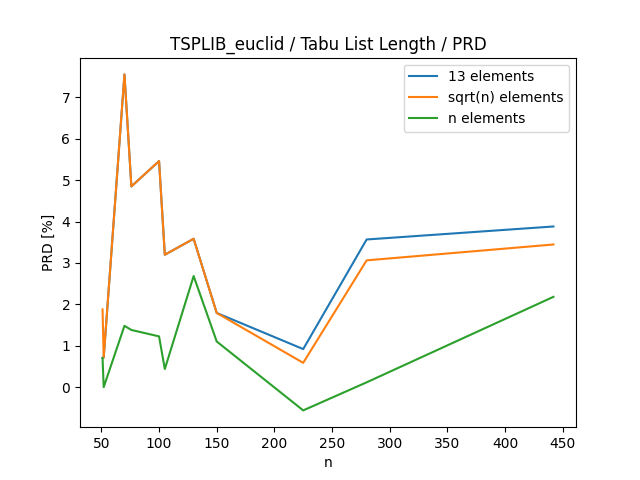
\includegraphics[width=\textwidth, 
                   height = 0.4\textheight, 
                   keepaspectratio]
                  {plots/tabu_tsplib_euclid_time} 
\end{center}


\subsection{Dane generowane przez nas}


\subsubsection{Grafy symetryczne}

\begin{center}
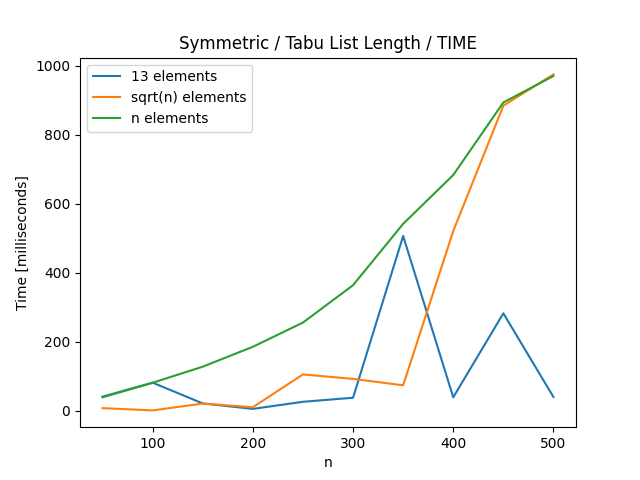
\includegraphics[width=\textwidth, 
                   height = 0.4\textheight, 
                   keepaspectratio]
                  {plots/tabu_symmetric_prd} 
\end{center}

\begin{center}
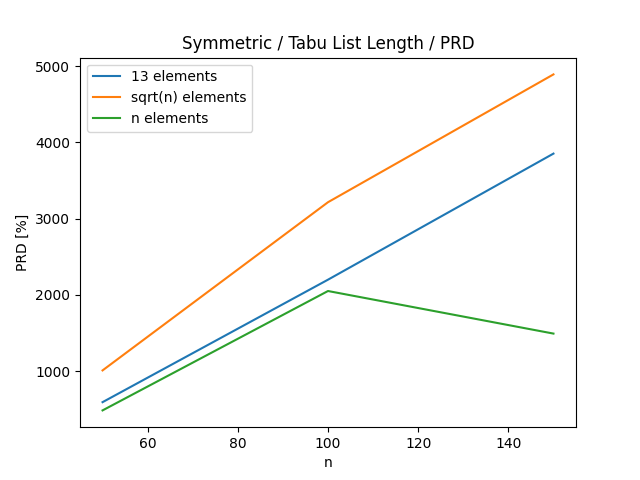
\includegraphics[width=\textwidth, 
                   height = 0.4\textheight, 
                   keepaspectratio]
                  {plots/tabu_symmetric_time} 
\end{center}

\subsubsection{Grafy asymetryczne}

\begin{center}
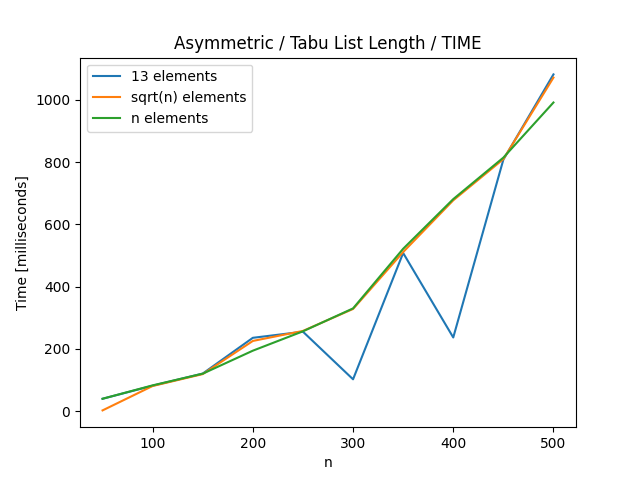
\includegraphics[width=\textwidth, 
                   height = 0.4\textheight, 
                   keepaspectratio]
                  {plots/tabu_asymmetric_prd} 
\end{center}

\begin{center}
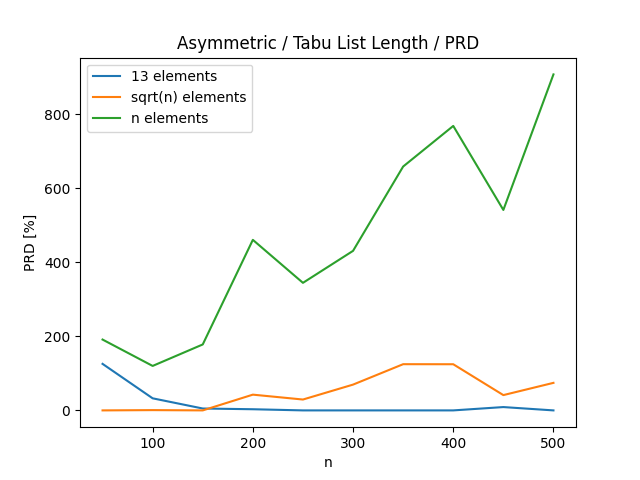
\includegraphics[width=\textwidth, 
                   height = 0.4\textheight, 
                   keepaspectratio]
                  {plots/tabu_asymmetric_time} 
\end{center}

\subsubsection{Grafy euklidesowe}

\begin{center}
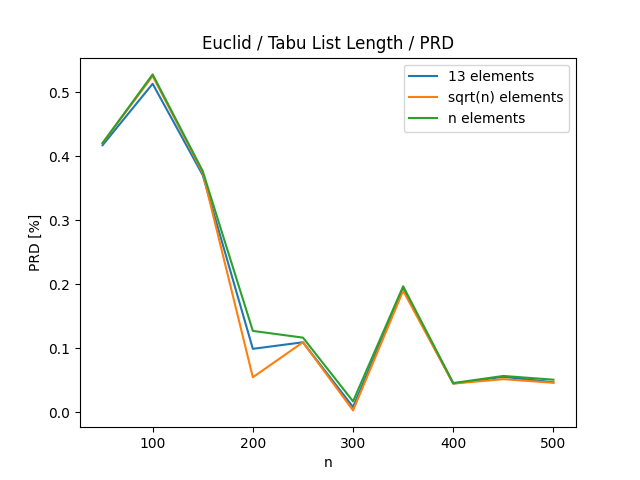
\includegraphics[width=\textwidth, 
                   height = 0.4\textheight, 
                   keepaspectratio]
                  {plots/tabu_euclid_prd} 
\end{center}

\begin{center}
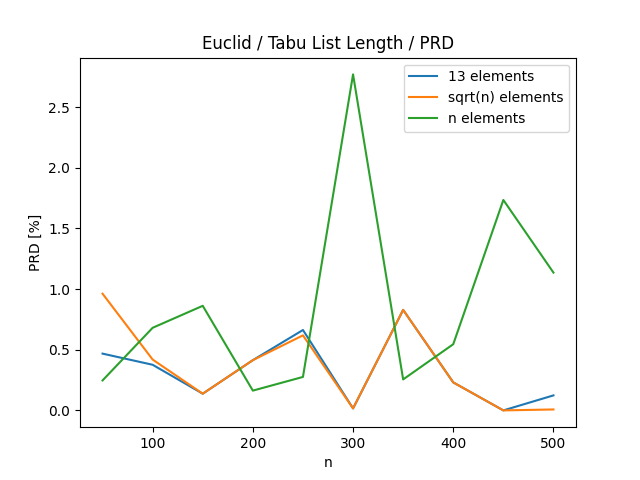
\includegraphics[width=\textwidth, 
                   height = 0.4\textheight, 
                   keepaspectratio]
                  {plots/tabu_euclid_time} 
\end{center}

\subsection{Obserwacje}

\subsection{Tabele}



\section{Porównanie sąsiedztwa insert i swap}

\subsection{Dane z TSPLIB}

\subsubsection{Grafy asymetryczne}

\begin{center}
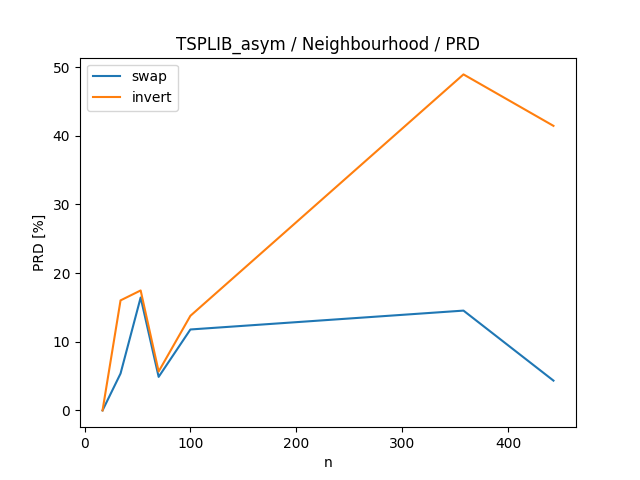
\includegraphics[width=\textwidth, 
                   height = 0.4\textheight, 
                   keepaspectratio]
                  {plots/neighbours_tsplib_asym_prd} 
\end{center}

\begin{center}
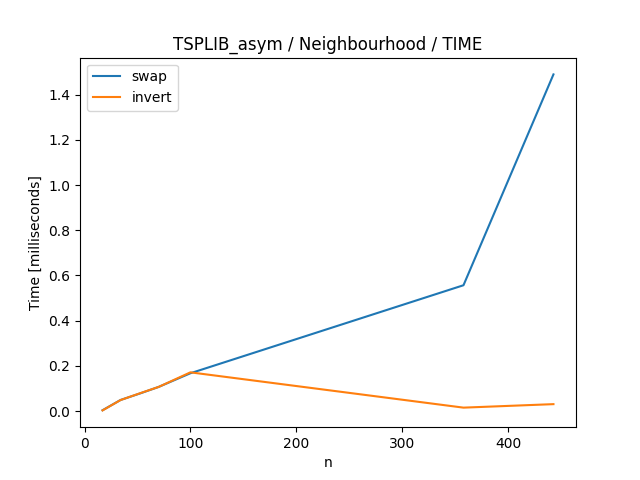
\includegraphics[width=\textwidth, 
                   height = 0.4\textheight, 
                   keepaspectratio]
                  {plots/neighbours_tsplib_asym_time} 
\end{center}

\subsubsection{Grafy euklidesowe}

\begin{center}
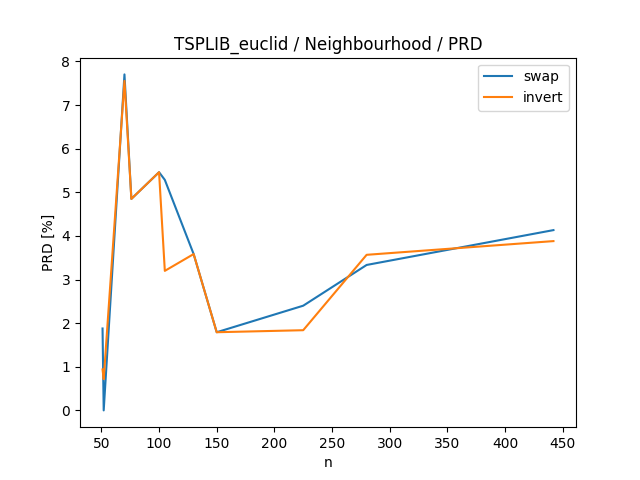
\includegraphics[width=\textwidth, 
                   height = 0.4\textheight, 
                   keepaspectratio]
                  {plots/neighbours_tsplib_euclid_prd} 
\end{center}

\begin{center}
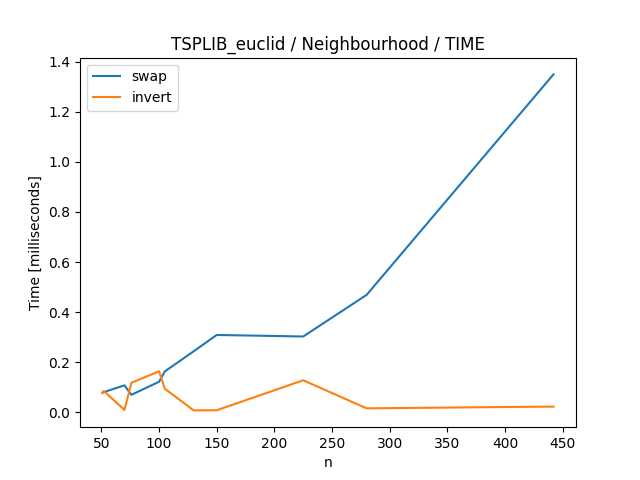
\includegraphics[width=\textwidth, 
                   height = 0.4\textheight, 
                   keepaspectratio]
                  {plots/neighbours_tsplib_euclid_time} 
\end{center}


\subsection{Dane generowane przez nas}


\subsubsection{Grafy symetryczne}

\begin{center}
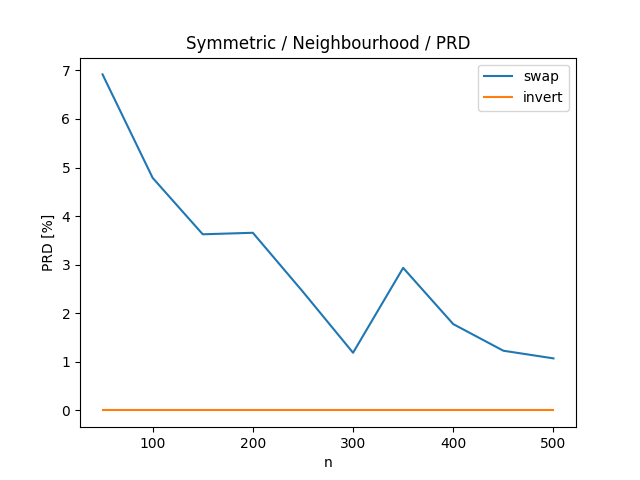
\includegraphics[width=\textwidth, 
                   height = 0.4\textheight, 
                   keepaspectratio]
                  {plots/neighbours_symmetric_prd} 
\end{center}

\begin{center}
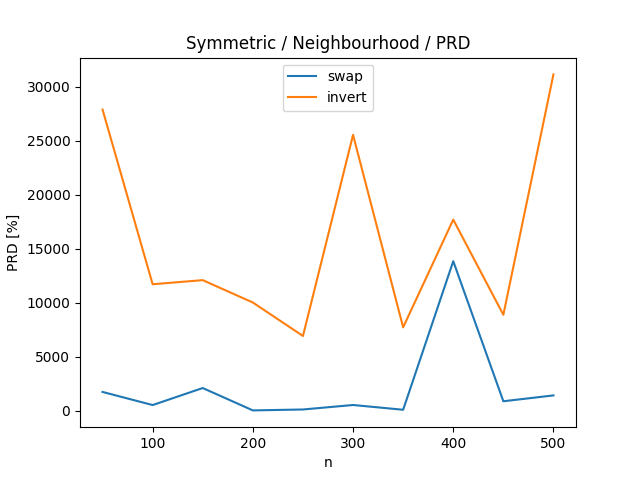
\includegraphics[width=\textwidth, 
                   height = 0.4\textheight, 
                   keepaspectratio]
                  {plots/neighbours_symmetric_time} 
\end{center}

\subsubsection{Grafy asymetryczne}

\begin{center}
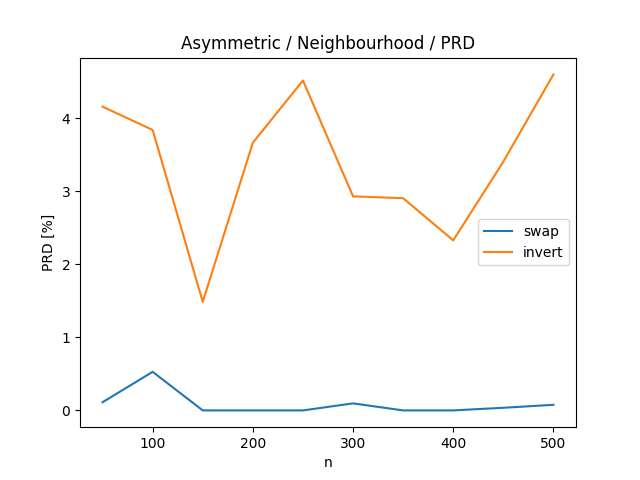
\includegraphics[width=\textwidth, 
                   height = 0.4\textheight, 
                   keepaspectratio]
                  {plots/neighbours_asymmetric_prd} 
\end{center}

\begin{center}
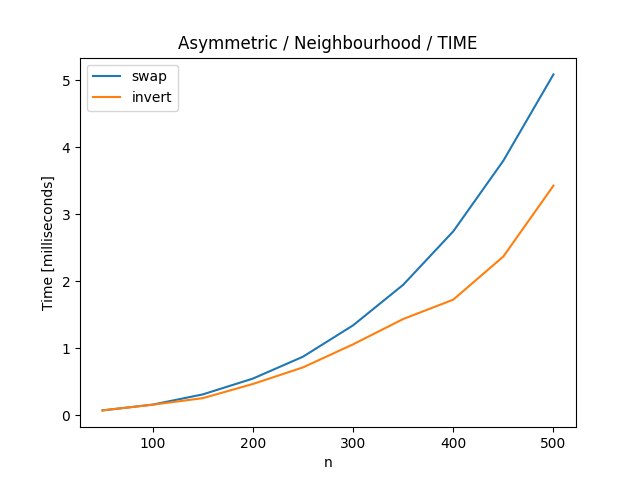
\includegraphics[width=\textwidth, 
                   height = 0.4\textheight, 
                   keepaspectratio]
                  {plots/neighbours_asymmetric_time} 
\end{center}

\subsubsection{Grafy euklidesowe}

\begin{center}
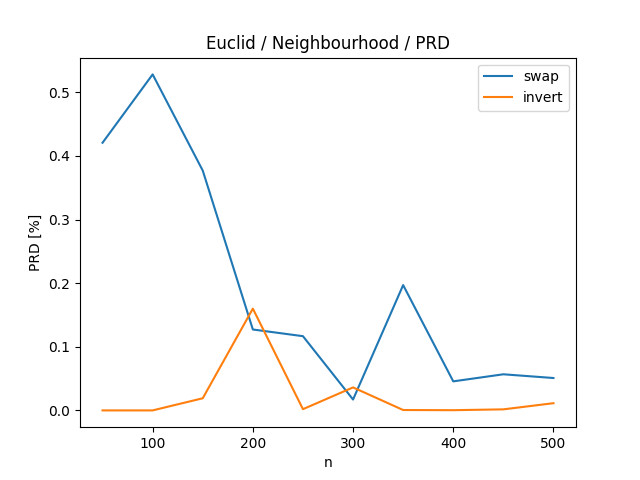
\includegraphics[width=\textwidth, 
                   height = 0.4\textheight, 
                   keepaspectratio]
                  {plots/neighbours_euclid_prd} 
\end{center}

\begin{center}
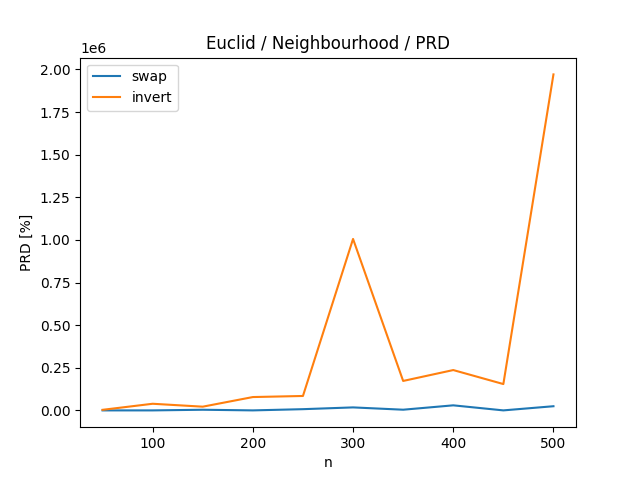
\includegraphics[width=\textwidth, 
                   height = 0.4\textheight, 
                   keepaspectratio]
                  {plots/neighbours_euclid_time} 
\end{center}

\subsection{Obserwacje}

\subsection{Tabele}



\section{Porównanie wersji wielowątkowej i wersji jednowątkowej}

\subsection{Dane z TSPLIB}

\subsubsection{Grafy asymetryczne}

\begin{center}
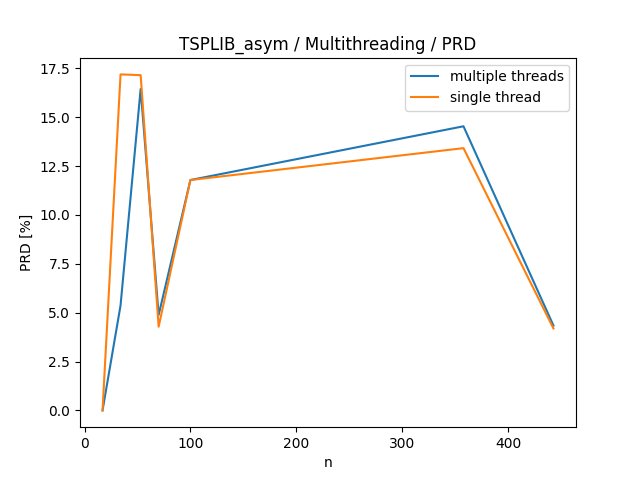
\includegraphics[width=\textwidth, 
                   height = 0.4\textheight, 
                   keepaspectratio]
                  {plots/multithreading_tsplib_asym_prd} 
\end{center}

\begin{center}
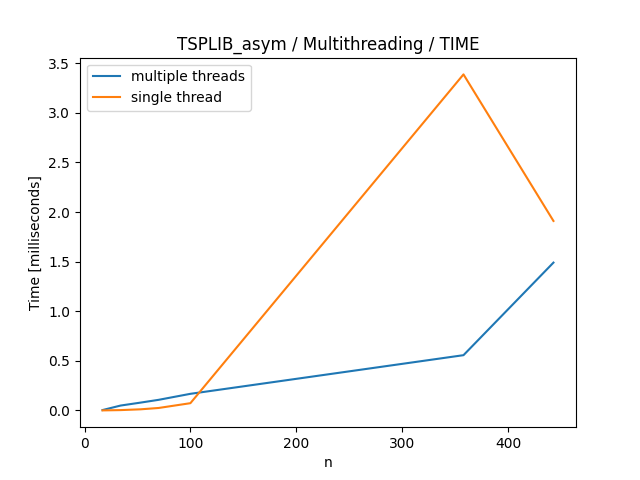
\includegraphics[width=\textwidth, 
                   height = 0.4\textheight, 
                   keepaspectratio]
                  {plots/multithreading_tsplib_asym_time} 
\end{center}

\subsubsection{Grafy euklidesowe}

\begin{center}
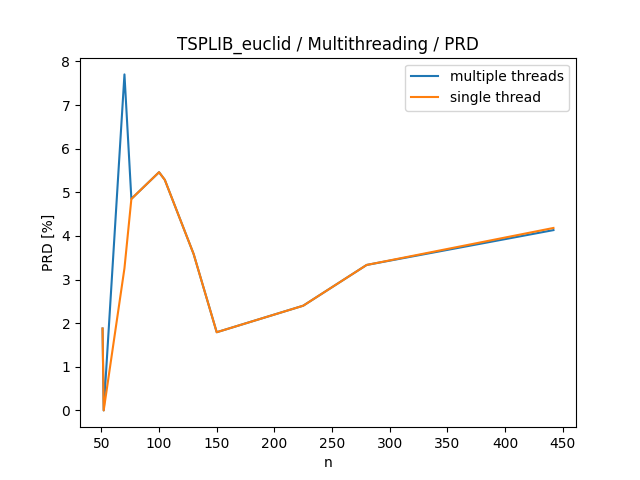
\includegraphics[width=\textwidth, 
                   height = 0.4\textheight, 
                   keepaspectratio]
                  {plots/multithreading_tsplib_euclid_prd} 
\end{center}

\begin{center}
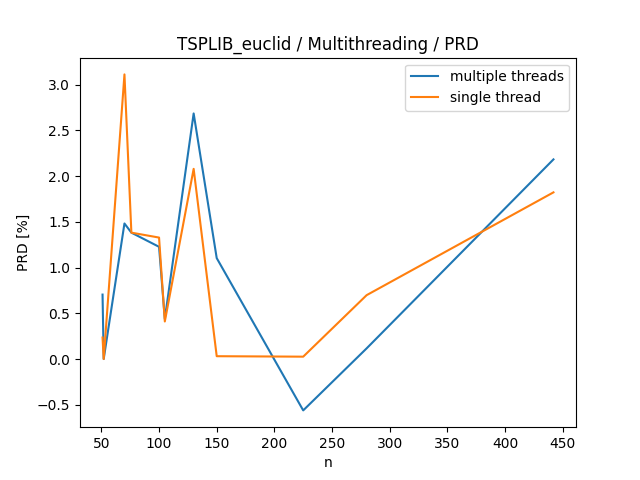
\includegraphics[width=\textwidth, 
                   height = 0.4\textheight, 
                   keepaspectratio]
                  {plots/multithreading_tsplib_euclid_time} 
\end{center}


\subsection{Dane generowane przez nas}


\subsubsection{Grafy symetryczne}

\begin{center}
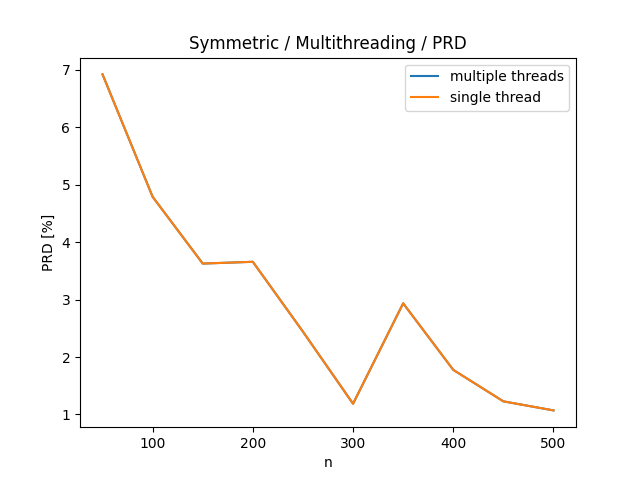
\includegraphics[width=\textwidth, 
                   height = 0.4\textheight, 
                   keepaspectratio]
                  {plots/multithreading_symmetric_prd} 
\end{center}

\begin{center}
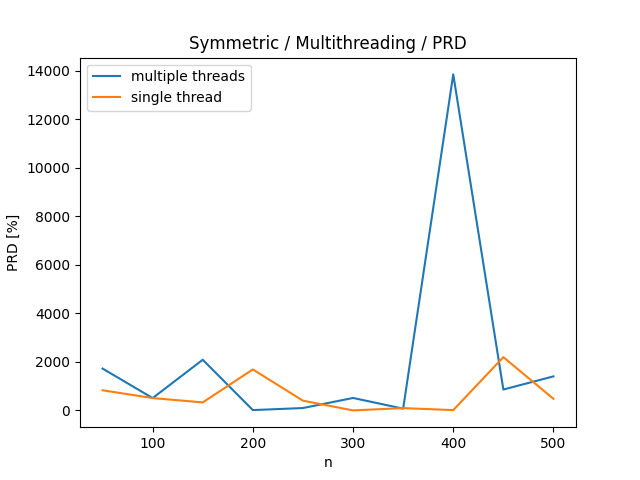
\includegraphics[width=\textwidth, 
                   height = 0.4\textheight, 
                   keepaspectratio]
                  {plots/multithreading_symmetric_time} 
\end{center}

\subsubsection{Grafy asymetryczne}

\begin{center}
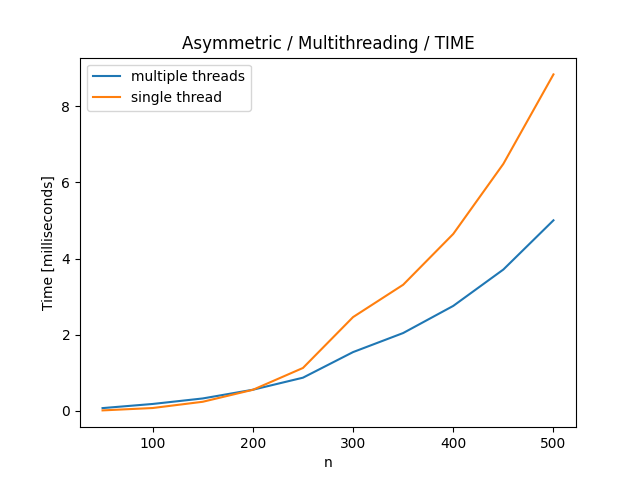
\includegraphics[width=\textwidth, 
                   height = 0.4\textheight, 
                   keepaspectratio]
                  {plots/multithreading_asymmetric_prd} 
\end{center}

\begin{center}
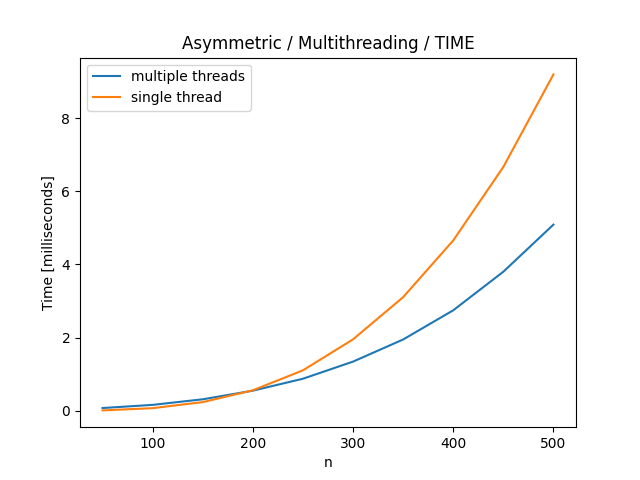
\includegraphics[width=\textwidth, 
                   height = 0.4\textheight, 
                   keepaspectratio]
                  {plots/multithreading_asymmetric_time} 
\end{center}

\subsubsection{Grafy euklidesowe}

\begin{center}
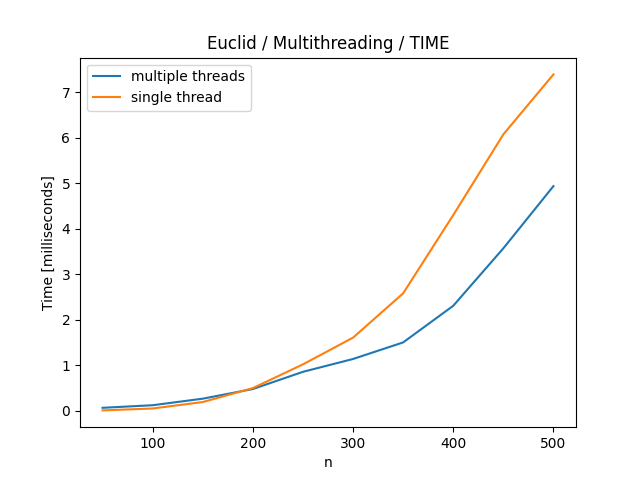
\includegraphics[width=\textwidth, 
                   height = 0.4\textheight, 
                   keepaspectratio]
                  {plots/multithreading_euclid_prd} 
\end{center}

\begin{center}
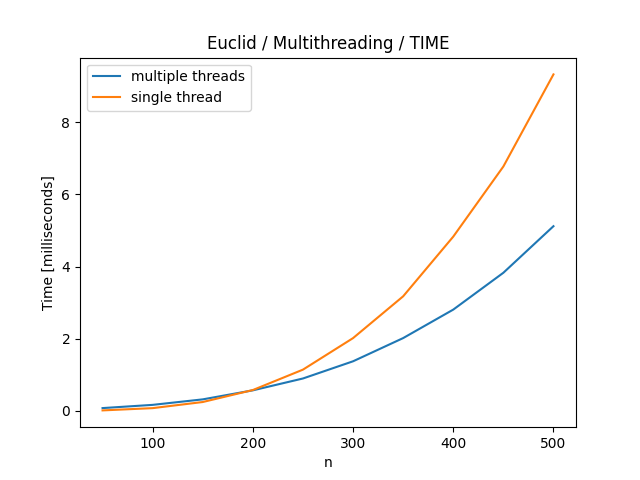
\includegraphics[width=\textwidth, 
                   height = 0.4\textheight, 
                   keepaspectratio]
                  {plots/multithreading_euclid_time} 
\end{center}

\subsection{Obserwacje}

\subsection{Tabele}



\section{Wnioski}

\end{document}